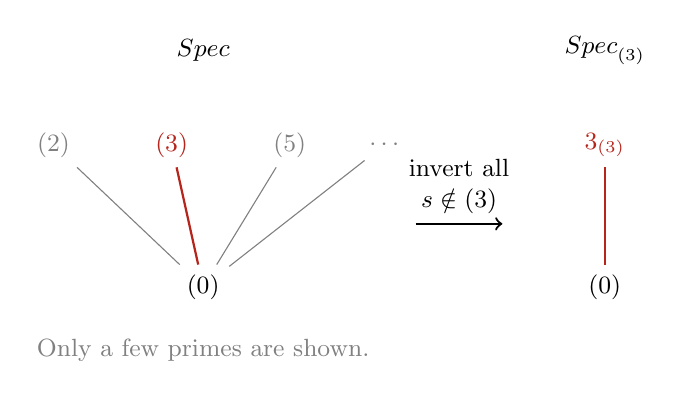
\begin{tikzpicture}[font=\small,x=1cm,y=1cm]
\node at (1.9,3.0) {$\operatorname{Spec}\Z$};
\node at (7.0,3.0) {$\operatorname{Spec}\Z_{(3)}$};
\node (z) at (1.9,0) {$(0)$};
\node[text=gray] (p2) at (0,1.8) {$(2)$};
\node[text=BrickRed] (p3) at (1.5,1.8) {$(3)$};
\node[text=gray] (p5) at (3,1.8) {$(5)$};
\node[text=gray] (more) at (4.2,1.8) {$\cdots$};
\draw[gray] (z)--(p2); \draw[BrickRed,thick] (z)--(p3);
\draw[gray] (z)--(p5); \draw[gray] (z)--(more);
\node (zz) at (7,0) {$(0)$};
\node[text=BrickRed] (pp) at (7,1.8) {$3\Z_{(3)}$};
\draw[BrickRed,thick] (zz)--(pp);
\draw[->,thick] (4.6,0.8)--node[above,align=center] {invert all\\$s\notin(3)$} (5.7,0.8);
\node[text=gray,align=center] at (1.9,-0.8) {Only a few primes are shown.};
\end{tikzpicture}
